Vi har udarbejdet følgende problemstilling, som danner grundlag for problemanalysen:

\textit{I en usikker tid, hvor mange danskere er økonomisk pressede, kan det være svært at holde styr på alle ens abonnementer, og det kan føre til økonomiske tab og stress. Hvordan kan vi hjælpe danskerne med at få bedre overblik over deres abonnementer og dermed mindske risikoen for økonomiske tab og stress?}

Problemstillingen ligger til grund for den , som vi vil gennemføre for at ydeliger identificere og forstå problemstillignens problem og årsag.

\subsection{Økonomiske udfordringer i samfundet}
Leveomkostningerne i Danmark er steget markant over en længere periode. Ifølge Danmarks Statistik havde Danmark allerede i 2024 forbrugerpriser, der lå 41 \% over det europæiske gennemsnit. Samtidig påvirker krig og geopolitisk uro konstant energi-, benzin- og dieselpriserne, hvilket har en betydelig indvirkning på den enkelte danskers økonomi – især for dem, der bor uden for de større byer, hvor mulighederne for offentlig transport er begrænsede.

I takt med de øgede levemokostninger i Danmark, bliver det også svære at finde frirum i økonomien til at spare sammen til f.eks. egen bolig eller bil i tætbeboede områder såsom København, hvor ejendomme, som f.eks. en etværelses lejlighed, kan koste op imod flere millioner kroner, er der ikke mange penge at gøre godt med.

Økonomiske uligheder i samfundet bliver også større jo længere ud på landet du kommer. Det påvirker økonomien, og gør det dermed sværere at have råd til de lidt dyrere leveomkostninger i Danmark. Vi har som gruppe tænkt os at undersøge følgende: Hvordan det økomomiske pres hos danskerne kan reduceres, samt gøre det muligt at overleve i de nuværende forbrugspriser uden at påvirke den individuelles levevilkår.

\begin{figure}[H]
    \centering
    \fbox{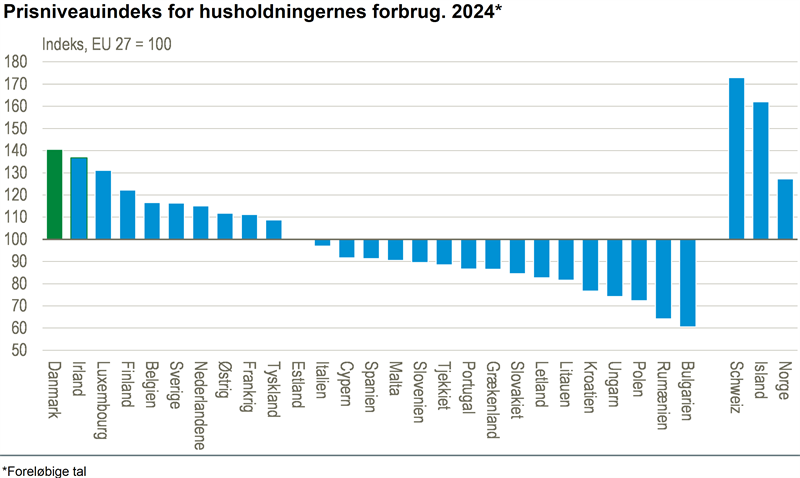
\includegraphics[width=0.8\textwidth]{assets/prisindeks.png}}
    \caption{Leveomkostninger i Danmark \footfullcite{Leveomkostninger2024}}
\end{figure}


\subsection{Abonnementers psykologiske effekter \label{sec:abpsef}}
Ud fra artiklen ”Understanding Subscription Models: \textit{»How Psychology Shapes
Customer Loyalty, Value Perception, and Cancellation Patterns«} \footfullcite{UnderstandingSubscriptionModels2025}, danner forfatteren et indblik i, hvordan strørre virksomhedder anvender psykologi til at påvirke, hvordan du opfatter dit abonnement, til at give dig en falsk fornemmelse af værdi. I artiklen bliver der beskrevet, hvordan personligt indforståelse af værdi påvirker individers sandsynlighed for at opsige et abonnement.

F.eks. grupperer virksomheder flere forskellige servicer som f.eks. streaming og musik + levering for en bestemt månedlig pris. Dette eksempel giver dig en fornemmelse af værdi for en højere pris. Dog bliver disse strategier primært anvendt for at give dig en fornemmelse af værdi, selv hvis du ikke anvender de yderligere grupperede fordele. I følgende analyse på næste side, kan det f.eks. ses, hvordan personer med abonnenter opfanger værdig, samt hvad der påvirker sandsynligheden for at opsige et abonnement ud fra den service som abonnementet tilbyder.

Ud fra Tabel 1 kan det ses, at de grupperede ydelser får procenten af folk til at opsige deres abonnementet ned på 12\% opsigelses lyst. Her ses det ligeledes, at forekommende prisstigninger har en opsigelses intention på 37\%, hvilket desuden er en af rødderne til vores nøgleproblem: Subscription fatigue.

\begin{table}[H]
\centering
\begin{tabularx}{\textwidth}{
    >{\raggedright\arraybackslash}X   % first column: left aligned flexible
    >{\centering\arraybackslash}m{3cm} % second column: centered fixed width
    >{\centering\arraybackslash}m{3cm} % third column: centered fixed width
    >{\raggedright\arraybackslash}X   % last column: flexible again
    }
    \toprule
    \rowcolor{gray!15}
    \textbf{Subscription Design} & 
    \textbf{Average Value Rating (1–5)} & 
    \textbf{Cancellation Intent (\%)} & 
    \textbf{Observed Psychological Effect} \\
    \midrule
    Bundled Services & 4.3 & 12\% & Framing $\rightarrow$ Enhanced Value \\
    Standalone Premium Tier & 3.7 & 24\% & Fairness Evaluation \\
    Frequent Price Increases & 3.1 & 37\% & Negative Affect, Loss Salience \\
    \bottomrule
\end{tabularx}
    \caption{Perceived Value by Subscription Design \footfullcite{UnderstandingSubscriptionModels2025}}
\end{table}

Både ud fra nogle forskellige strategier til at få folk til at beholde deres abonnementer.

Du kan se de Grupperede Ydelser får procenten af folk til at opsige deres abonnoment
ned på 12\% opsigelses lyst, hvor at forkommende pristigninger har en opsigelses
intetion på 37\%, dette er en af røderne til vores nøgle problem: Subscription fatigue

Herefter har vi også en virksomheds baseret grådighed, ved abonnomenter ejer du
aldrig det du betaler for, hvilket vil sige at virksomhederne har 100\% ejerskab over det
produkt du har købt.

I artiklen “The Subscription Economy and Its Contribution to the Global Economy” skrevet af Paula Cobazaru, som er Assistant Professor, phd studerende ved Alexandru Loan Cuza University Og Alexandru Tugui, som er professor ved Alexandru Loan Cuza University
bliver der beskrevet, at gennemsnitligt betaler den individuelle forbruger 133\$ om måneden på abonnementer som vil svare til 853,43 DKK om måneden, hvilket svarer til ca 10266,79 DKK om året pr. forbruger, med en estimeret stigning på 18\% om året. Og hvis man så tager det til sammenligning til hele jordens befolkning, vil det lægge den estimerede markedsværdi inden for abonnementer på cirka 1,5 trillion dollars, eller 9.624.300.000.000 DKK.

Hvilket betyder abonnementer har fået en meget større økonomisk og global betydning, og at den globale markedsværdi konstant vil stige.

Da virksomhederne får muligheder for at styre udbud og efterspørgelse selv, kan de selv styre hvor meget der ryger ind og ud af markedet. Dette danner et kæmpe problem for den gennemsnitlige forbruger, da individet ikke har noget ejerskab eller kontrol. Virksomheder kan også bruge disse abonnementer til at danne faste relationer med kunderne, hvilket gør at individet har svære ved at få kontrol over egen kapital. Dette fører derfor til Subscription fatigue, hvor individet ikke har nogle form for overblik over deres abonnementer og økonomi til et punkt hvor forbrugeren ikke agerer på deres økonomi længere.


\subsection{Subscription fatigue}
Subscription fatigue på dansk »abonnementsudmattelse«, som er den mentale og økonomiske tilstand, der opstår, når en forbruger føler sig overvældet af antallet af løbende betalinger og tjenester, som de skal administrere. I denne rapport anvender vi begrebet som en »diagnose« af et moderne samfundsproblem, hvor den teknologiske udvikling har gjort det for nemt at starte et abonnement, men for uoverskueligt at vedligeholde eller opsige det.


Hvorfor opstår Subscription fatigue? 


Subscription Fatigue opstår typisk på grund af tre hovedfaktorer:\footfullcite{subFatt}
\begin{enumerate}
    \item \textbf{Kognitiv overbelastning:}\\
    Forbrugeren mister overblikket over, hvilket tjenester de reelt har adgang til, og hvilket de bruger. Når hver tjeneste kræver sit egent login, app og betalingsaftale, ophører abonnementet med at være en bekvemmelighed og bliver i sted et en administrativ byrde. 
    \item \textbf{Økonomisk »leaking«:}\\
    forbrugeren oplever små månedlige beløb, som virker ret ubetydelige hver for sig, men samlet så dræner de privatøkonomien (jf. afsnit \ref{sec:abpsef} om det gennemsnitlige forbrug på 853 kr./md.). Dette skaber helt underbevidst en stressfaktor, da man ved, pengene forsvinder til forbrug, men ikke præcis hvorhen.
    \item \textbf{Beslutningslammelse:}\\
    Som beskrevet i afsnit \ref{sec:abpsef}, bruger virksomheder psykologiske tricks som bundling. Dette gør det svært for brugeren at vurdere den reelle værdi af tjenesten, hvilket fører til, at man beholder et abonnement "for en sikkerheds skyld", selvom man sjældent bruger det. 
\end{enumerate}
 
Vores fokus i dette projekt er ikke blot at identificere Subscription fatigue, men at udvikle et teknologisk værktøj, der kan hjælpe med at modkæmpe det. Ved at automatisere overblikket kan vi fjerne den kognitive belastning fra individet og derved forbedre både deres økonomiske råderum og deres livskvalitet.
 